\documentclass{article}
\usepackage[utf8]{inputenc}
\usepackage{graphicx,wrapfig,lipsum}
\usepackage{caption,subcaption}
\usepackage[a4paper]{geometry}
\usepackage{amsfonts}
\usepackage{fancyhdr}
\usepackage{amsmath}
\usepackage{graphics}
\usepackage{verbatim}
\usepackage{hyperref}
\usepackage[table,xcdraw]{xcolor}
\usepackage[normalem]{ulem}
\usepackage{float}
\useunder{\uline}{\ul}{}
\hypersetup{
    colorlinks=true,
    linkcolor=blue,
    filecolor=magenta,      
    urlcolor=cyan,
}
 
\urlstyle{same}

%\title{Report kmlmm}
%\author{Pietro Fronte}
%\author{david}
%\date{December 2018}

\pagestyle{fancy}
\lhead{Pietro Fronte}
\chead{David Manubens}
\rhead{Asaf Badouh}
\cfoot{Page \thepage}
\renewcommand{\headrulewidth}{0.4pt}
\renewcommand{\footrulewidth}{0.4pt}

\title{Half-term Project - Kernel Methods\\Image classification}

\author{Pietro Fronte \\ David Manubens\\Asaf Badouh }
\date{\today}

\begin{document}

\maketitle
\section{Abstract}
Image classification problems usually imply a multi-class classification problem with high dimensional input data. Traditional classification methods are shown to generalize poorly on this kind of problems. One of the advantages of SVM is their good generalization performance, which is because it is a maximum margin classifier, that is making it more robust to outliers and noise. Therefore, it may outperform traditional classification methods like logistic regression or LDA in techniques such as image classification. In this project we will test SVM based image classification with the \textbf{Caltech 101}\cite{LiFergusPerona04} images dataset. From one side, we will test a couple of methods for image feature extraction that have proven to be robust for computer vision tasks, and then we will apply SVM classifier on the obtained features and try to tweak the kernel function and SVM hyperparameters to obtain the best possible accuracy on the classification.


\section{Introduction}
Image classification has been around for many years now. Still, as a subpart of computer vision, it is nowadays one topic of high interest, due to the increasing number of images available on the web and the amount of information we can obtain from them.  Therefore, we have chosen to apply SVM techniques to Image classification problem, to both gain experience in applying SVM to a practical real-life problem, and at the same time, to get some idea of the main challenges of computer vision. 
Images of $N\times M$ pixels, each pixel belonging to $[0..255]$ or $[0..1]$, can be represented as a vector $x \in \mathbb{R}^{N\cdot M}$. Then, any classifier we use will take this vector as input for each image. The problem of this representation for images is that images that are very similar to the human eye, can be treated as very different when measured by a pixel-wise distance measure like the Euclidean norm (See Figure[\ref{fig:handwrite}]).  The reason for this is that that pixel-wise representation lacks of invariance with respect to some transformations that human eye is able to detect as similar. Some of these transformation include translations, (small) rotations, (small) changes in size, blur, brightness and contrast (See Figure[\ref{fig:handwriteinvar}]) are factors that humans typically consider irrelevant when judging if two images show the same object. 
\begin{figure}[!h]
    \centering
    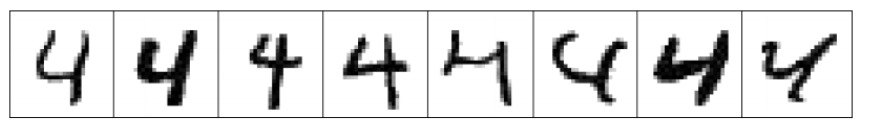
\includegraphics[width=0.9\textwidth]{Images/handwrite4.jpg}
    \caption{Handwritten digit 4 - different appearances}
    \label{fig:handwrite}
\end{figure}
\begin{figure}[!h]
    \centering
    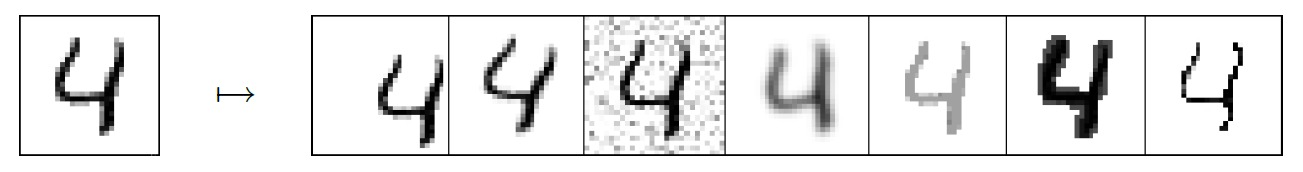
\includegraphics[width=0.9\textwidth]{Images/handwrite4transformations.jpg}
    \caption{Handwritten digit 4 - different transformations}
    \label{fig:handwriteinvar}
\end{figure}
How to deal with this variance in images has been extensively studied in computer vision field. Mainly, there are four options to deal with it. 
\begin{itemize}
    \item Extending the training set. 
    \item Normalization of the image. 
    \item Integrating invariance in the kernel. 
    \item Finding invariant features representations. 
\end{itemize}

The most widely developed and effective approach so far has been to find invariant features representation. In our project, we will combine two invariant representations: the gradient representation and the histogram representation. Combined, they are what is called Histogram of Gradients representation in Computer Vision literature. These two representations will be explained more in depth in the \textit{Theory section}[\ref{section:theory}]. Depending on the granularity at which histograms of gradients are obtained, more grained or less grained representations of the image can be obtained (See Figure[\ref{fig:hog_levels}]). So, one of the points we will study is which is the optimal representation of the image in terms level of granularity at which histograms of gradients will be computed. 

\begin{figure}[!h]
    \centering
    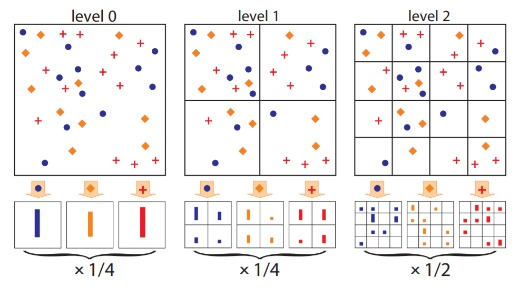
\includegraphics[width=0.9\textwidth]{Images/hog_levels.jpg}
    \caption{Example of constructing a pyramid for L = 2}
    \label{fig:hog_levels}
\end{figure}

On the other side, we want to test the capability of SVM to fit and generalize the feature invariant representations that we have obtained with the histograms of gradients. For this we will try the generalization performance of several different kernels such as the linear kernel or the RBF kernel. We will run several experiments and try to explain why some kernels generalize better depending on the chosen HOG representations. For instance, we may find that for representations with HOG obtained at level 0 of the image (See Figure[\ref{fig:hog_levels}]), the radial kernel outperforms the others, while for representations with HOG obtained at level 2, the linear kernel outperform the others.

As for the dataset, we have chosen the \textbf{Caltech 101} images dataset that contains images classified in 101 categories, each category having different number of images. In order to avoid problems derived from imbalanced datasets, we have decided to to keep only the categories that have 70 or plus images, resulting in 31 categories. For the purpose of interpretability of results, this may be too much categories. Ideally, we would like to have a smaller subset of categories but that are different in nature, meaning that some of them are hard to classifiy and some are easy. To select categories that meet this criteria, we have launched a classification with a linear SVM and the 31 categories, obtaining the Specificity for each of the categories:

\begin{table}[H]
\centering
\begin{tabular}{|c|c|}
\hline
\textbf{Class}& \textbf{Sensitivity}      \\ \hline
{car\_side}        & {1}    \\ \hline
{trilobite}        & {1}    \\ \hline
{airplanes}        & {0.95} \\ \hline
{minaret}          & {0.95} \\ \hline
{ketch}            & {0.9}  \\ \hline
{Motorbikes}       & {0.9}  \\ \hline
{Faces}            & {0.8}  \\ \hline
{grand\_piano}     & {0.75} \\ \hline
{helicopter}       & {0.75} \\ \hline
{Leopards}         & {0.75} \\ \hline
{revolver}         & {0.7}  \\ \hline
{chandelier}       & {0.65} \\ \hline
{ewer}             & {0.65} \\ \hline
{laptop}           & {0.65} \\ \hline
{watch}            & {0.65} \\ \hline
\end{tabular}
\centering
\begin{tabular}{|c|c|}
\hline
\textbf{Class}& \textbf{Sensitivity}      \\ \hline
{bonsai}           & {0.6}  \\ \hline
{electric\_guitar} & {0.6}  \\ \hline
{menorah}          & {0.6}  \\ \hline
{sunflower}        & {0.6}  \\ \hline
{umbrella}         & {0.6}  \\ \hline
{brain}            & {0.55} \\ \hline
{buddha}           & {0.55} \\ \hline
{butterfly}        & {0.55} \\ \hline
{crab}             & {0.55} \\ \hline
{kangaroo}         & {0.55} \\ \hline
{llama}            & {0.55} \\ \hline
{hawksbill}        & {0.5}  \\ \hline
{ibis}             & {0.45} \\ \hline
{scorpion}         & {0.3}  \\ \hline
{starfish}         & {0.3}   \\ \hline
\end{tabular}
\end{table}

So, we have selected some "easy" categories, some "medium" and some "hard", up to 10. The chosen ones will be: scorpion, starfish, airplanes, bonsai, faces, minaret, motorbikes, trilobite, umbrella, watch. So this results in 10 classes, with 70 images per class. 


\section{Previous Work}
Invariant features descriptions have been used and studies extensively in Computer Vision field. Histograms of colours are used in \cite{SVM_VC}, together with SVM to perform Image classification, with good accuracy results. Studies done in \cite{dalal2005histograms} prove the efficiency of HOG as invariant representation of images for pedestrian detection. Other popular methods of invariant representation like SIFT are described in \cite{DavidG}.  From this simple representations, more complex representations have been explored by combining or adding granularity layers, such as in [\cite{Spatial_Pyramid}, \cite{grauman2007pyramid}], where spatials pyramids of HOGS are used. More complex feature representations of images such as the Pyramid of HOGs imply that the feature representation is no longer a vector in R, and thus traditional kernels like linear or RBF kernels are not useful anymore. This leads to explore the use of alternative kernels such as the Pyramid Match Kernel [\cite{grauman2007pyramid}], that are able to deal with hierarchical representations of images with HOGs.
With respect to the use of SVM and kernelized methods for image recognition, there is also a lot of literature, mostly between 2000 where firsts good results were obtained for image classification [\cite{SVM_VC}] and 2010 or so, when Deep Learning proved to be more efficient for Computer visions. The most advanced methods using kernels for image processing are methods that use kernels which rather than taking a vector as input, are able to process hierarchical structures of data that are able to represent the inherent hierarchical nature of an image [\cite{Spatial_Pyramid},\cite{grauman2007pyramid}, \cite{bosch2007representing}]. 





\section{Theory}\label{section:theory}

 
The theory behind the work we did can be divided into 2 macro categories: 
Preprocessing: from a .png image to a vector containing numerical features of the image
Modelling : from vector of numerical features to the final prediction

\subsection{Preprocessing}    

Once loaded the images in workspace, they appear as a 3D matrix: 2 dimensions for the height and width of the image (the length of these 2 components vary depending on the dimensions in pixels of the image) and the third dimension is a fixed vector of 3 components storing the RGB components of each pixel. \newline

From this structure we want to extract the so-called \textit{feature descriptor}, or in other words a numerical representation of the same image by extracting useful information from it. Generally a feature descriptor can belongs to two different macro categories:
\begin{itemize}
    \item \textbf{Global feature descriptor}: retrieve useful information from the entire object(image). Contour representations, shape descriptors and texture features belong to Global features descriptors. HOG (histogram of gradients ) and Shape Matrices are examples of algorithm that belong to this category.
    \item \textbf{Local feature descriptor}: it doesn't focus on the whole image but try to describe patches (key points in the image) of an object. SIFT(Scale-invariant feature transform) and SURF (Speeded Up Robust Feature) are examples of algorithm that belong to local descriptors category.
\end{itemize}

For our task (Multi-class Classification of images) we chose to adopt the Histogram of Gradient as feature descriptor of our images.

\subsubsection {The idea behind the Histogram of Gradients}

When we see an image, from a human point of view, we are able to distinguish different objects in the same image mainly because of their shapes, their color or their position in the image, and thanks to our experience (we touched it, we saw it, we were in that place and so on..) we are also able recognize them. Computers, in this case, have no experience with real life and no eyes to see images. To let them “see” the image and help them recognize objects we try to, as said before, highlight the different shapes that characterize a particular object and make it different from the others. This is what actually Histogram of gradient does.

The basic idea is that a local object presence and shape is well approximated by the local distribution of gradient intensity and direction. This is because gradients magnitude is large around edges and corners (regions of intensity changes) so thanks to that we are able to highlight shapes of object. 
\subsubsection{ HOG Evaluation}
\begin{minipage}{0.5\textwidth}
To evaluate the Histogram of Gradient we evaluate first the derivatives with respect to X and Y axis - process achieved by filtering the image with the following kernels (Figure [\ref{xy_filters}]). Once evaluated the two components we can build the magnitude of the gradient (Equation[\ref{eq:gradient}]) and the direction(Equation[\ref{eq:direction}]) of the same.
\begin{equation}\label{eq:gradient}
G = \sqrt{(g_x^2 + g_y^2)}
\end{equation}
\begin{equation}\label{eq:direction}
\theta = \arctan \frac{g_y}{g_x}
\end{equation}
With $g_x$ and $g_y$ the first derivatives with respect to x and y axis.
\end{minipage}
\begin{minipage}{0.5\textwidth}
\begin{figure}[H]
    \centering
    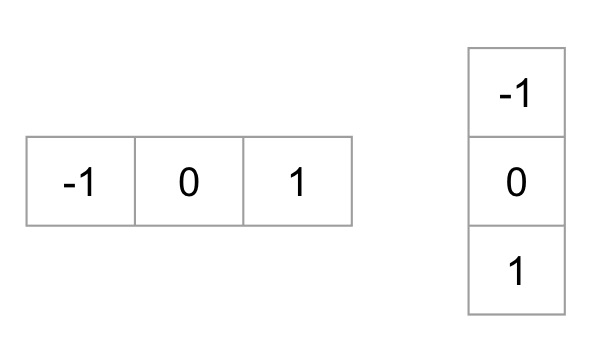
\includegraphics[width=0.9\textwidth]{Images/gradient-kernels.jpg}
    \caption{X, Y Filters.}
    \label{xy_filters}
\end{figure}
\end{minipage}

Once we know how to evaluate the gradient we need to understand where to evaluate it. 
We split first the current image into a number of squared cells, each cell is composed by a $n\times n$ pixels. Remember that each pixel contains also the RGB components so at the end each cell end up having $n\times n \times 3$ values!

On each of these squared cell we are going to evaluate the histogram of gradients. So from 1 cell we will get $n\times n \times 2$ (direction and magnitude) values that we will redistribute in an histogram with h number of bins.

% fix image dimensions %
\begin{figure}[H]
\centering
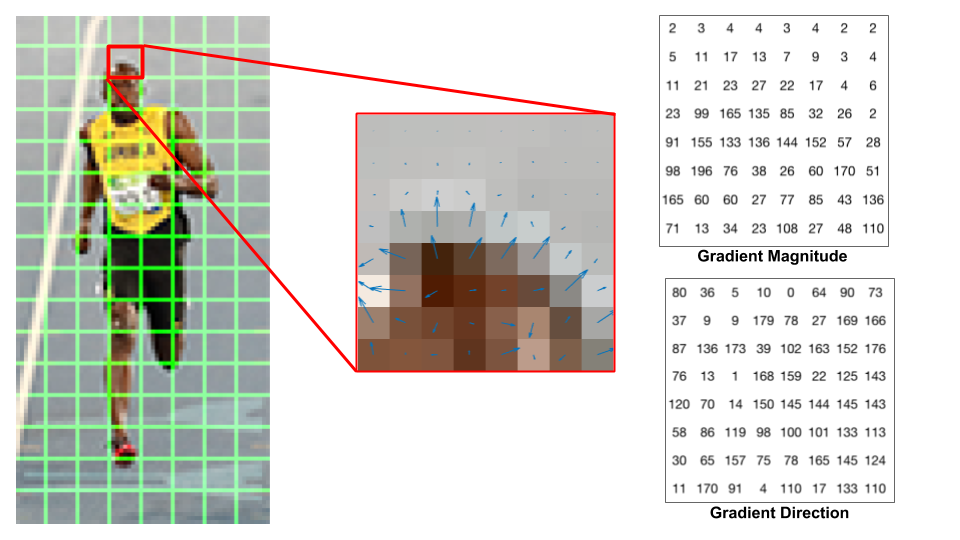
\includegraphics[width = 0.9\linewidth]{Images/hog-cell-gradients.png}
\caption{Example HOG in Cell}
\end{figure}

% fix image dimensions %
\begin{figure}[H]
\centering
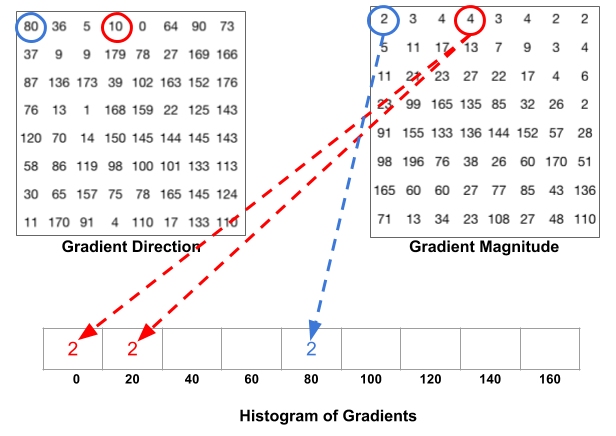
\includegraphics[width = 0.8\linewidth]{Images/hog-histogram-1.png}
\caption{Example HOG in Cell}
\end{figure}

% fix image dimensions %
\begin{figure}[H]
\centering
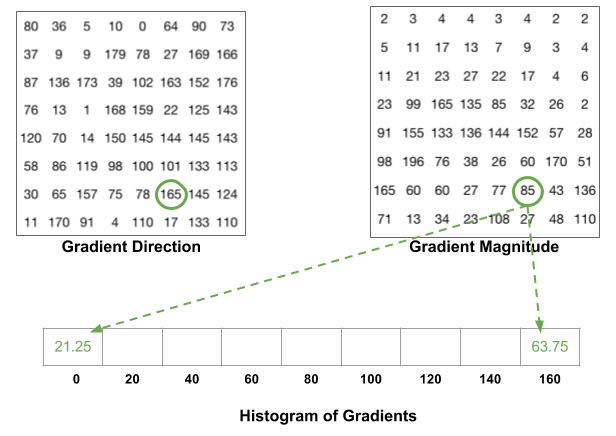
\includegraphics[width = 0.8\linewidth]{Images/hog-histogram-2.png}
\caption{Example HOG in Cell}
\end{figure}



For this reason, what comes out from HOG evaluated in a cell is just a vector of length h (number of bins). Concatenating each of this vectors of length h coming out from each cell we will get the feature descriptor vector based on Histogram of Gradients. If we split and image into m cells then we will end up having a descriptor of length $m\cdot h$.

\subsection{Modelling} 

Once built the feature descriptor vector we are ready to start the modelling part. 
The idea is to use a kernelized version of Support Vector Machine to carry our multi-class classification task.
SVM is one of the most used Machine Learning algorithm in classification task. 
\begin{itemize}
    \item Given a dataset D = \{($x_1$,$t_1$), ... , ($x_n$,$t_n$)\} with $x_i$ $\epsilon$ ${\rm I\!R}^d$ and $t_i \epsilon \{ -1; +1\}$ \\
    \item Given a separating hyperplane f(x) = $w^Tx$ = b with w = \{$w_1$,...$w_n$\} and b variable \\
    \item Given the support vectors of the hyperplane 
    \begin{itemize} 
    \item SV1: $w^Tx$ = b+1 \\ 
    \item SV2: $w^Tx$ = b-1
    \end{itemize}
    and the distance between them $\frac{2}{||w||}$
    \item Given a set of slack variable $\varepsilon_i$ with $\varepsilon$ = \{$\varepsilon_1$, ... , $\varepsilon_n$\} and a parameter C 
\end{itemize}

Then the primal SVM formulation is:
\[
min_{w,b} f(x) = \frac{1}{2} w^Tw + C \sum_{i=1}^n \varepsilon_i \\
\text{subject to: } t_i(w^Tx-b)+\varepsilon_i \geq 1
\]

However this does not allow us to introduce any kernel. For this reason we need to move to the dual version of SVM problem first to see appear an inner product of the variable matrix x.

\begin{itemize}
    \item Given a set of variable $\alpha$ = \{ $\alpha_1$, ..., $\alpha_n$ \} \\
    \item Given a dataset D = \{($x_1$,$t_1$), ... , ($x_n$,$t_n$)\} with $x_i$ $\epsilon$ ${\rm I\!R}^d$ and $t_i \epsilon \{ -1; +1\}$
\end{itemize}

The dual version of a SVM problem is:

\begin{equation}\label{eq:min}
\begin{split}
min_\alpha f(x) =& \sum_{i=1}^n \alpha_i -\frac{1}{2} \sum_{i=1}^n \sum_{j=1}^n \alpha_i \alpha_j t_i t_j \langle x_i,x_j\rangle  \\\\[-1em]
\text{subject to: }& 0 \leq \alpha_i \leq C \quad 1\leq  i\leq n \\\\[-1em] 
&\sum_{i=1}^n \alpha_i t_i = 0
\end{split}
\end{equation}

In this way we are now able to substitute the inner product with a kernel function. Why use a kernel function inside and exploit the kernel trick?
This is because our points may be (almost surely) non linearly separable. Thus a reasonable way out is to increase the space dimension through a mapping function $\phi$ such that $\phi$ : ${\rm I\!R}^d \longrightarrow {\rm I\!R}^z $ with d $\leq$ z, and in the new dimension being able to classify them with a linear classifier (hyperplane).

\subsubsection{Kernels}
What is a kernel and why we use it? \\
K(x,x') = $\langle \phi(x), \phi(x) \rangle$
Through the kernel matrix we can now introduce inside the problem information about dissimilarity measure between data points in order to have a better classification.


\begin{itemize}
    \item Polynomial kernel : K(x,x') = $\langle \phi(x), \phi(x) \rangle^y$ 
    \item RBF kernel : K(x,x') = exp(-$\gamma||x_i - x_j||^2$) $\text{ with } \gamma=\frac{1}{2\sigma^2}$
\end{itemize}


\section{Experiments}
\subsection{Experimental Methodology}
In order to carry out our experiments we mainly used the caret(classification and regression training) R package\cite{caret}. 
The function train() from the above package allow us to build a model based on tuning parameter process. 
The tuning of the parameters is performed by cross validation, in particular is a repeated Cross Validation of type 3x5-folds. For each parameter the automated tuning parameter try 5 different values, it means that if the model has p parameters the number of combination it'll try are $5^p$. Based on the maximum Accuracy obtained for each combination it'll pick the set of best parameters.
Once found the needed parameters it builds the model to use for prediction. What we evaluate at the end is the general accuracy of the classification task.

We focused on SVM classifiers in 3 different setup: 
\begin{enumerate}
    \item Simple SVM - Linear kernel
    \item Kernelized SVM - Polynomial kernel
    \item Kernelized SVM - RBF kernel
\end{enumerate}

When passing to train() function of caret package the names "svmLinear", "svmPoly", "svmRadial" we are calling the SVM implementation of the R package $kernlab$\cite{Kernelab}. 
The parameters found with cross validation are:
\begin{enumerate}
    \item For linear kernel: C cost of constraint violation
    \item For polynomial kernel : degree of the polynomial, C cost of constraint violation and scale
    \item For RBF kernel : $\gamma$ parameter and C cost of constraint violation
\end{enumerate}
The values of train and test set are scaled, before modelling process

\subsection{Experiment 1 - Optimal HOG Parameters}
As explained in the \textit{Theory section}[\ref{section:theory}] HOG has two parameters to be tuned:
\begin{itemize}
    \item Number of splits -  number of image partitions.
    \item Number of bins - size of the histogram
\end{itemize}

Let's try to get an intuition on how these parameters will affect the performance. If we just use 1 split, we will be taking the image as a whole. The more splits, the more partitions of the image we will have. If we consider the image as a whole, we will achieve in variance with respect to translations, rotations. However, we will loose the ability to get more grained knowledge, meaning that local part of the image that could be very informative in terms of identifications will be lost when taken together with the rest of the image.
On the other side, if we make a lots of splits in an image, the image will be less invariant to translations or rotations, but each split will allow to capture better the details of that part of the image. So in summary, we would say that the optimal number of splits depends highly on the kind of images. 
Regarding the number of bins, the effect is similar to that of the number of bins. Less umber of bins will make classification more robust to rotations, but at the cost of losing some details that can be important in terms of recognizing the image. 

In this experiment, we will try several combinations of splits and bins, in order to see if there is any combination or values that do provide significant better accuracy. 

The parameters of this experiment are:
\begin{enumerate}
    \item Number of splits = 2, 5, 8, 11, 14, 17
    \item Number of bins = 6, 10, 14, 18, 22.
    \item Number of images per category = 70
    \item Number of classes = 10
    \item Kernel = Linear, Radial. 
\end{enumerate}

The results are the following:

\begin{figure}[H]
    \centering\begin{subfigure}[H]{0.49\linewidth}
    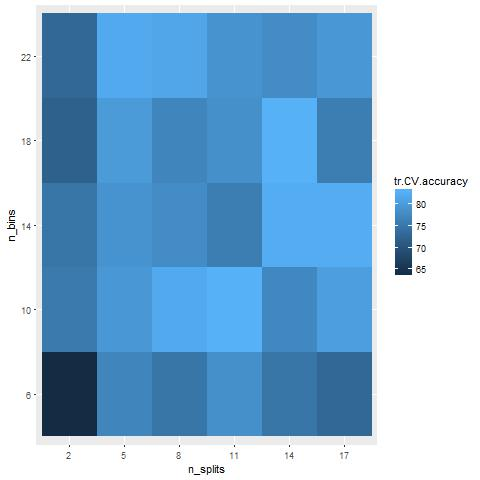
\includegraphics[width=\textwidth]{Images/Accuracy_for_categories_starfish_minaret.jpeg}
    \caption{Linear Kernel}
    \label{subfig:linear}
    \end{subfigure}
    \centering\begin{subfigure}[H]{0.49\linewidth}
    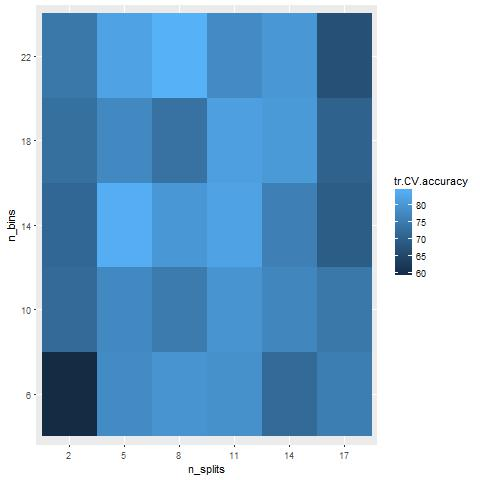
\includegraphics[width=\textwidth]{Images/Accuracy_for_categories_starfish_minaret_radial.jpeg}
    \caption{Radial kernel}
    \label{subfig:radial}
    \end{subfigure}
    \caption{Accuracy results for different HOG parameters}
    \label{fig:exp1}
\end{figure}

The conclusions that we can draw from the above results are the following. From one side, 2 splits seems to be too few, meaning that if we split the image in 4 pieces, we do not have enough specific information about concrete part of the image that are important. However, from 5 to 17 splits, there is no evidence of improvement or deterioration of the accuracy. This would mean that with the given images, if we split the image in 25 parts, we have enough details in order to have information about important parts of the image. On the other side, the fact that having a the image split in 17*17 parts does not deteriorate the performance, means that we should not find a lot of translations and rotations or objects of different sizes in the images. If we explore a bit the dataset, we will see that this is generally true: 


\begin{figure}[H]
    \centering
    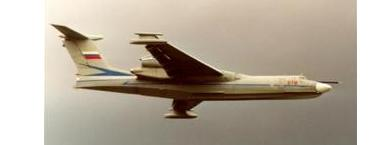
\includegraphics[width=0.3\textwidth]{Images/airplane_1.jpg}
    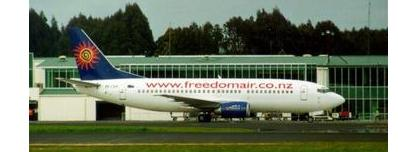
\includegraphics[width=0.3\textwidth]{Images/airplane_2.jpg}
    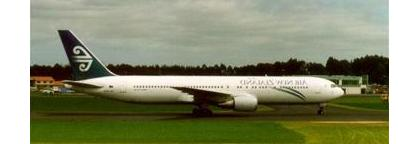
\includegraphics[width=0.3\textwidth]{Images/airplane_3.jpg}
    \caption{Airplane category}
    \label{fig:airplane}
\end{figure}

\begin{figure}[H]
    \centering
    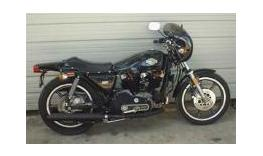
\includegraphics[width=0.3\textwidth]{Images/moto1.jpg}
    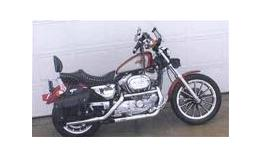
\includegraphics[width=0.3\textwidth]{Images/moto2.jpg}
    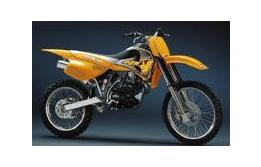
\includegraphics[width=0.3\textwidth]{Images/moto3.jpg}
    \caption{Motorbikes category}
    \label{fig:moto}
\end{figure}

Finally, comparing the results of the linear kernel and the radial kernel, we can see that there are no significant differences. The only thing we see is that with 17 splits, the accuracy in the radial kernel decreases. This may be due to the fact that as radial kernel is able to fit perfectly the data and thus, if we have a very high dimensional feature space, like with 17 splits and 22 bins (17*17*22 = 6538 dimensions), the radial kernel may be over fitting the data. 


In the next experiment, we will see explore if by combining 2 HOG, each of them with different number of binds and different number of splits provides any improvement in the accuracy obtained. 

\subsection{Experiment 2 - Two HOGs Features vector}
After exploring different combinations of $split\times bin\_size$ we wanted to explore the possibilities of creating features vector the comprised from two HOGs. For our experiment, we used the the following setting:

The parameters of this experiment are:
\begin{enumerate}
    \item $HOG_1$ parameters combination = \{4\_6, 6\_6, 8\_6 , 4\_12, 6\_12, 8\_12\}
    \item $HOG_2$ parameters combination = \{10\_6, 12\_6, 14\_6, 16\_6, 10\_12, 12\_12, 14\_12, 16\_12\}
    \item Number of images per category = 70
    \item Number of classes = 10
    \item Kernel = Linear 
\end{enumerate}

We created different features vector combinations by concatenate $HOG_1$ and $HOG_2$ into one features vector, for example, $Features\_vector_{HOG_{11},HOG_{21}} = ((4\_6), (10\_6))$, later we used the "Linear Kernel" to check the performance of the different combination. In figure[\ref{fig:exp1a}] we can see the performance of our classifier. The numbers the axis stands for hog configuration ($HOG(Split\_Bins)$) and the gradient of color stands for the accuracy(\textbf{Note}: the darker blue, the better accuracy). 

\begin{figure}[!h]
    \centering
    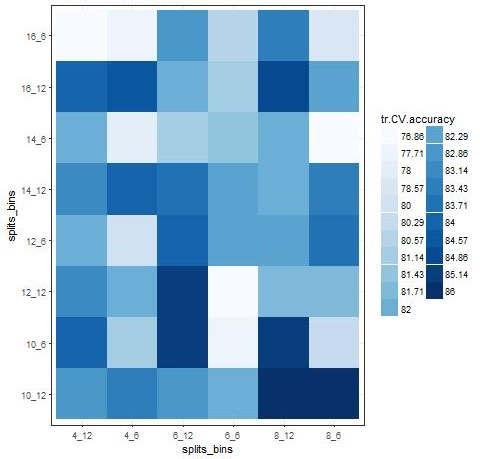
\includegraphics[width=0.6\textwidth]{Images/Accuracy_for_categories_1a.jpeg}
    \caption{Accuracy of Split and Bin combination with linear kernel}
    \label{fig:exp1a}
\end{figure}

From figure[\ref{fig:exp1a}] we can learn, again, that it's hard to draw conclusions for the "right" combination.
\begin{itemize}
    \item Two combinations get 86\% accuracy: $F_1: (8\_6, 10\_12)$ and $F_2: (8\_12,10\_12)$
    \item Three combination get 85.14\% accuracy: $F_3:(6\_12, 10\_6)$, $F_4:(8\_12, 10\_6)$ and \\ $F_5:(6\_12, 12\_12)$
\end{itemize}

Our intuition from the experiment is that HOG with big bin (=12) will be work better with both small and big bin. In case HOG with big bin combined with Hog with small bin, the small bin should have relative high split. This intuition can be used only as \textit{rule of thumb} as we can see, for example, the combination of $HOG(14\_12)$ with $HOG(8\_6)$ perform better than with $HOG(6\_8)$, however, the combination with $HOG(4\_6)$ outperform the bigger split.

The conclusion from the experiment is that in order to get better quality features vector combination we need to apply more complicated technique such as "Spatial Pyramid Matching" as suggested in \cite{Spatial_Pyramid}. Since extending the features vector is costly in power computing (for our poor laptops) and the performance just slightly improved, we decided to stick with one HOG as features vector.

\subsection{Experiment 3 - Dynamically Grows Dataset By Adding Classes}

This experiment is conducted with the aim of understating what is the behavior/performance of each classifier in a dataset that grows dynamically. It means that each classifier is tested first in a dataset of just 2 classes (binary classification) and at each step we will add 1 more class to the dataset in order to check not only the classifier performance over the whole dataset but also the performance of each classifier  with respect to a single class. 
The parameters of this experiment are:
\begin{enumerate}
    \item Number of splits = 4
    \item Number of bins = 15
    \item Number of images per category = 70
    \item Number of classes = 10
\end{enumerate}
Each feature descriptor vector will have length $4\times4\times15 = 240$, 700 images in total.\\

% left minipage%
\begin{minipage}{0.45\textwidth}

\begin{table}[H]
\scalebox{0.8}{
\begin{tabular}{|l|l|l|l|}
\hline
\textit{Sensitivity}        & Linear        & Polynomial        & RBF         \\ \hline
\rowcolor[HTML]{FFFC9E} 
2. Starfish *               & 0,77          & 0.61              & 0.72        \\ \hline
2. Minaret *                & 1             & 0.94              & 1           \\ \hline
\rowcolor[HTML]{FFFC9E} 
3. Bonsai                   & 0.94          & 0.77              & 0,72        \\ \hline
\rowcolor[HTML]{FFFC9E} 
4. Scorpion                 & 0.44          & 0.66              & 0.44        \\ \hline
5. Motorbikes               & 1             & 1                 & 1           \\ \hline
\rowcolor[HTML]{FFFC9E} 
6. Faces                    & 1             & 0.94              & 0.88        \\ \hline
7. Watch                    & 0.83          & 0.83              & 0.83        \\ \hline
7. Airplanes                & 0.94          & 1                 & 1           \\ \hline
9. Umbrella                 & 0,88          & 0,83              & 0.83        \\ \hline
10. Trilobite               & 1             & 1                 & 1           \\ \hline
\multicolumn{4}{|l|}{* These to classes are the first used in the first step} \\ \hline
\end{tabular}
}
\caption{Sensitivity over classifiers}
\label{table:sens}
\end{table}

\end{minipage}
%right minipage%
\begin{minipage}{0.55\textwidth}
\begin{figure}[H]
\centering
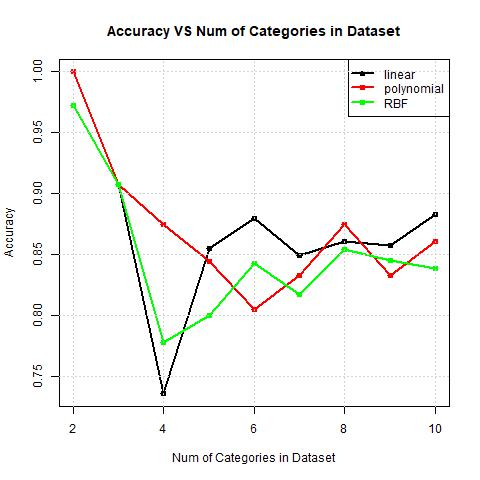
\includegraphics[width=0.9\textwidth]{Images/Number_categories_vs_accuracystarfish_minaret.jpeg}
\caption{Accuracy VS Num Categories}
\label{fig:exp3}
\end{figure}
\end{minipage}

Checking the results above(Table[\ref{table:sens}], Figure[\ref{fig:exp3}]) we can see that generally a linear kernel perform better than the others, sometimes gaining a gap greater than a 20\%. Interesting is the behavior of the classifiers in the class $4. Scorpion$. It seems a complicated class to understand, a class where RBF and linear SVM fail completely (even going under 0.5 of sensitivity) while the polynomial manage to do something better catching a 0.66 in sensitivity (however still an overall low value compared with the other class).

\subsection{Experiment 4 - Kernels Function Comparison}

In this section, we will compare the performance of the SVM with several different kernel functions. In theory, if the 10 classes are not linearly separable, we should see an increase of performance when using RBF kernel or Polynomial Kernel instead of Linear Kernel. However, after having run experiments up to now, we have not seen such behaviour. anyways let's set up an experiment to check it. In this case, as we want to enforce full classes separability, we will not use \textit{caret} to train the SVM, but we will force the parameter C to 100 to penalize the miss-classification errors and ensure full separability. We will also try different number of images to see if there is any dependency on the training size for any kernel. 

\begin{enumerate}
    \item Number of splits = 4
    \item Number of bins = 15
    \item Number of images per category = 15, 30, 45, 60, 70
    \item Cost = 100
    \item Number of classes = 10
    \item Kernels = Linear, Polynomial 2, Polynomial 3, RBF, LaplacianRBF.  
\end{enumerate}

The results are the following.

\begin{figure}[H]
\centering
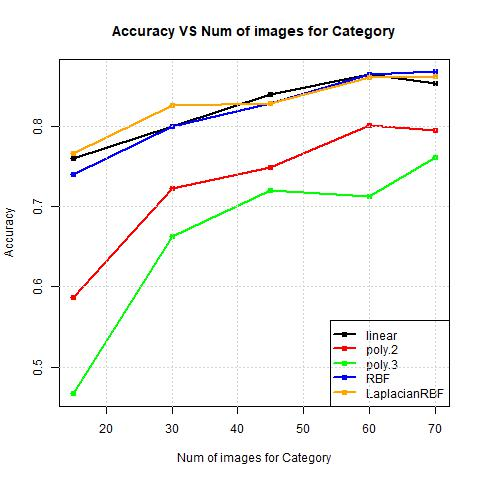
\includegraphics[width=0.7\textwidth]{Images/Kernel Methods.jpeg}
\caption{Accuracy for different kernel functions}
\end{figure}

As we can see, the thee linear, RBF and Laplacian RBF kernel functions have very similar performance for all training data sets sizes used. Considering that we have set C parameter to 100 and we have leaved the sigma parameter to default, the fact that we have similar performance with radial kernels and linear kernels tells us that there is a linear classifier that gives full separability of the data, in the feature space dimensions we are working at. Thus, there is no need for non-linear feature space transformations provided by the radial kernel functions. We will discuss more in depth this point in the conclusions. 


\subsection{Experiment 5 - Comparison With Traditional Methods}

As mentioned in the introduction, SVM are expected to have a better generalization performance with problems in high dimensional spaces than traditional methods. In this experiment we will compare the performance of the following methods: Naive Bayes, Classification Tree, LDA, KNN. All of them will be trained automatically using Caret Package, and compared with a SVM with both Linear Kernel and RBF kernel. 

\begin{enumerate}
    \item Number of splits = 4
    \item Number of bins = 15
    \item Number of images per category = 15
    \item Number of classes = 10
\end{enumerate}

The results are the following:

\begin{figure}[H]
\centering
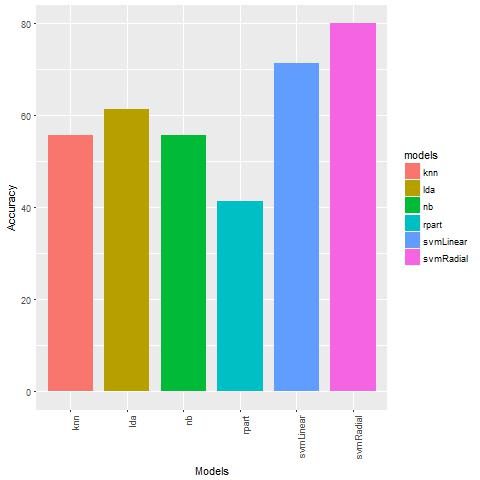
\includegraphics[width=0.7\textwidth]{Images/Accuracy_for_categories_starfish_minaret_2.jpeg}
\caption{Accuracy for different methods}
\end{figure}

As we can see, SVM outperforms the other methods, by at least 10 percent. However, here we have used only 15 images. It would be interesting to see the evolution if we use more data to train the methods. 

Next, we will execute all 6 models with different number of images, to see how the differences change when adding different number of images:

\begin{enumerate}
    \item Number of splits = 4
    \item Number of bins = 15, 30, 45, 60, 70
    \item Number of images per category = 15
    \item Number of classes = 10
\end{enumerate}

The results are the following:

\begin{figure}[H]
\centering
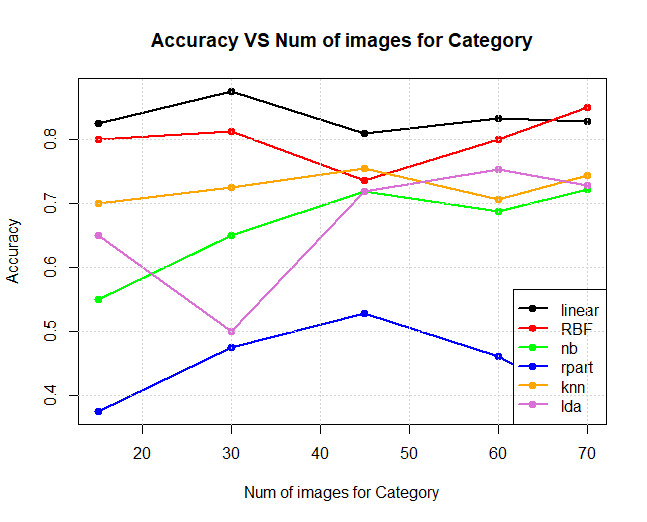
\includegraphics[width=0.6\textwidth]{Images/WhatsApp.jpeg}
\caption{Accuracy vs num category by method}
\end{figure}

As we saw in the previous plot, with 15 images, the SVM with 80 \% accuracy methods have at least 10 accuracy points more than next method which is KNN with 70 \%, while other methods range from 37\% for classification tree to 65\% of linear discriminant. While increasing the number of images, we see that methods like the Naive Bayes or the Linear discriminant get up to 70 \% of accuracy, same as KNN but none of them reaches the 80\% of the support vector machines. Thus, we confirm that even with little data, the generalization performance of the support vectors is much better, as it is more robust to outliers or any other points that may appear when adding more data. As expected, the generalization performance of other methods improves with more data (except with the classification tree), but does not reach the accuracy obtained with SVM even with much less data. 

\subsection{Experiment 6 - Dynamically Grows Classes in Dataset} \label{experiment_6}
In this experiment we want to investigate what happens when we increase the number of images, once fixed the number of categories and the parameters to build the HOG for each image. 
The steps chosen to perform this task are 15, 30, 45, 60, 70. We stop at 70 because there are categories with no more than 70 photos.
The other parameters are set to the following values:
\begin{enumerate}
    \item Number of splits = 4
    \item Number of bins = 15
    \item Number of classes = 10
    \item Classes :  Bonsai, Motorbikes, Scorpion, Faces,  Umbrella, Airplanes, Trilobite, Watch, Starfish, Minaret
\end{enumerate}

The aim of this experiment is to check if there is any relation between the number of images in the dataset to classify and the classifier (kernelized, not kernelized, etc..)

\begin{figure}[H]
\centering
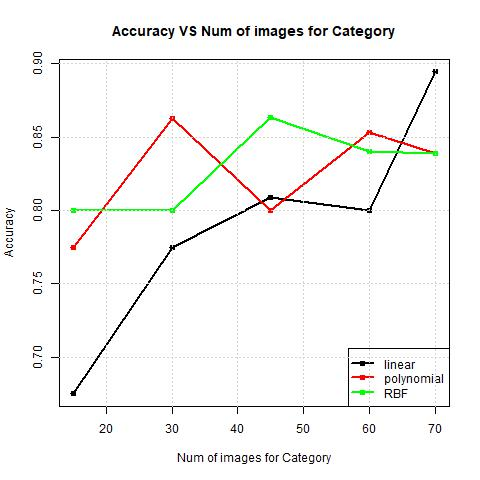
\includegraphics[width=0.6\textwidth]{Images/Accuracy_for_categories_bonsai_Motorbikes.jpeg}
\caption{Accuracy VS Num Images}
\end{figure}

Looking at the plot we can't state an exact conclusion, we are aware that the number of images may be low so actually we don't know what happens when the images are like 150 per category. Generally we can only state that the trend is positive for all the classifier, all of them increase the accuracy increasing the number of images fed into the classifier. 

\section{Conclusions}
The general idea of this work was to learn about computer vision basics, test SVM as classifier for images and check any possible differences between the linear version and the kernelized versions of this algorithm.

From preprocessing part we learn how an Histogram of Gradient works and and translate an image in a vector of numerical information. We tried to investigate more about the connection between parameters and accuracy, how they can affect, in a better or worst way my classification task. Even if not a state of art method to encode images information we are quite satisfied of the results obtained with this descriptor.

From modelling part we played around to get some interesting conclusion about how kernelized version would act against a normal support vector machine. We didn't find any clear proof to state that a RBF or polynomial version of SVM perform better than a linear kernel (especially when number of instances is way smaller than the number of features) even if there are works that proof the contrary.\cite{hsu2003practical}
We than wanted to compare the SVM as classifier against other algorithm. We expected SVM to be a very good classifier in images classification and actually we got clear results on this topic. 

However we got an idea on why we didn't find any concrete results on RBF kernel on SVM. We know that RBF kernel help us distinguish datapoints when the number of feature is not enough to build a linear classifier ( in this case an hyperplane ) to classify them correctly. For that reason, applying RBF and mapping the datapoints in an higher feature space, a linear classifier can perform better. However in this case the number of feature we are building may be larger enough to allow linear SVM to classify them correctly; also looking at the images per-se we notice that they are "easy" recognizable ( same position in the picture, same profile, same background, etc ) making the pictures so different between categories that even just a linear SVM is able to do a good job.

\section{Future Work}
Due to the lack of computing power we could not run a full experiments based on the whole dataset or try various datasets. There are other options to create features vector for image representation that can be explored, such as color histograms-based or Invariant feature mapping \cite{lampert2009kernel}. 
we have elided discussion of deep learning and neural network methodologies as it will be the second half of the half-term project. However, it will be interesting to compare the accuracy and time performances of the models. In addition, in experiment 6[\ref{experiment_6}] we compare the performance of SVM with different number of images in the chosen categories. Since we know that SVM preform good with (reletivly) small dataset, it will be interesting to extend this experiment with larger categories size and add neural network methodologies. Our intuition is that while using small category size SVM will outperform NN, NN will outperform SVM as the category size grows.

\newpage
\nocite{*}
\bibliographystyle{unsrt}
\bibliography{references}
\end{document}
